\documentclass[11pt,a4paper]{article}
\usepackage[margin=0.9in]{geometry}
\usepackage{graphicx}
\usepackage{booktabs}
\usepackage{caption}
\usepackage{subcaption}
\usepackage{xcolor}
\usepackage{hyperref}
\usepackage{microtype}

\hypersetup{
  colorlinks=true,
  linkcolor=black,
  citecolor=black,
  urlcolor=blue!60!black
}

\title{\textbf{TimeSeriesFlow and AdaptiveForecast}\\[0.4em]\large Comparative Evaluation and Commercial Impact Report}
\author{TimeSeriesFlow Open Benchmark}
\date{2026-06-15}

\begin{document}
\maketitle

\begin{abstract}
We benchmark four entity processing approaches on three public multi-entity time series datasets.
This Phase 1 report answers a single question: should you adopt TimeSeriesFlow, AdaptiveForecast,
or the combined stack for your workload? We measure screening throughput, gate outcomes, routing
diversity, and orchestration overhead. We do \textbf{not} yet measure forecast accuracy (Phase 2).
Vanilla pandas wins on raw speed for simple statistics. AdaptiveForecast blocks unfit entities and
assigns model families. TimeSeriesFlow adds batch structure with modest overhead on lightweight work.
\end{abstract}


\section{Executive verdict}
\noindent\textbf{Bottom line.} Across 40 entities, TimeSeriesFlow is an orchestration layer (\textasciitilde{}14x pandas on stats-only work), AdaptiveForecast adds screening and routing on Intel Berkeley Lab, ETT Hourly (ETTh1), and forecast accuracy remains unmeasured. UCI Household Power blocked every entity under current gates (screening worked; not a deployment-ready forecast slice). Full-stack screening averages 60 entities/s.

\subsection{When to use the stack}
\begin{itemize}
  \item Entity count is large enough that manual loops, retries, and progress matter
  \item Entity quality varies and some series should be blocked before training
  \item A single global model family is risky and per-entity routing is required
  \item You accept profiling overhead in exchange for screening and orchestration
\end{itemize}

\subsection{When not to use the stack}
\begin{itemize}
  \item You only need exploratory mean, count, or simple aggregates on a small fleet
  \item All entities are homogeneous and pass the same model family
  \item You must prove forecast accuracy gains (not measured in Phase 1)
  \item Raw pandas throughput is the primary success metric
\end{itemize}

\subsection{Effectiveness decision table}
\begin{table}[htbp]
\centering
\caption{Pass or fail against benchmark criteria (Phase 1: no forecast accuracy test).}
\label{tab:decision}
\small
\begin{tabular}{p{4.8cm}cccc}
\toprule
Criterion & Pandas & TSFlow & AF loop & Full stack \\
\midrule
Faster than pandas for the same lightweight stats task & Pass & Partial & Fail & Fail \\
Blocks unfit entities before model training & N/A & N/A & Pass & Pass \\
Assigns different model families per entity & N/A & N/A & Pass & Pass \\
Forecast accuracy better than a single global model & N/A & N/A & Not tested & Not tested \\
Production batch ops (checkpoints, parallel workers, retries) & Fail & Not tested & N/A & Not tested \\
Screening throughput for nightly fleet batches & N/A & N/A & Partial & Partial \\
\bottomrule
\end{tabular}
\end{table}

\noindent\textbf{Notes.}
\begin{itemize}
  \item \textbf{Faster than pandas for the same lightweight stats task}: TimeSeriesFlow adds a mean 13.6x slowdown on stats-only work; profiling dominates full-stack cost.
  \item \textbf{Blocks unfit entities before model training}: 5 of 40 entities blocked portfolio-wide. All entities blocked on: UCI Household Power.
  \item \textbf{Assigns different model families per entity}: Mean routing diversity 7.0\%; up to 2 unique families assigned.
  \item \textbf{Forecast accuracy better than a single global model}: Phase 2 backtest not run. No MAE or sMAPE in this report.
  \item \textbf{Production batch ops (checkpoints, parallel workers, retries)}: Benchmark used workers=1 and did not exercise checkpoint resume.
  \item \textbf{Screening throughput for nightly fleet batches}: Mean full-stack screening: 59.6 entities/s.
\end{itemize}


\subsection{TimeSeriesFlow}
\noindent\textbf{Verdict (Pass):}
Effective as an orchestration layer (14x slower than pandas on the same lightweight stats task; acceptable overhead for batch structure).

\textbf{Use when:}
\begin{itemize}
  \item Structured per-entity batch runs with retries and progress hooks
  \item Teams that outgrow ad-hoc groupby loops but do not need profiling yet
\end{itemize}

\textbf{Do not use when:}
\begin{itemize}
  \item Beating pandas on simple mean and row-count aggregates
  \item Proving forecast quality (orchestration only in this benchmark)
\end{itemize}

\subsection{AdaptiveForecast}
\noindent\textbf{Verdict (Partial):}
Partially effective: screening blocks unfit entities before training; routing assigns multiple model families where patterns differ; on UCI Household Power all entities failed gates (short span slice; screening-only outcome). Forecast accuracy was not tested.

\textbf{Use when:}
\begin{itemize}
  \item Screening entities that fail quality gates before training spend
  \item Routing labels when entity patterns differ within a fleet
\end{itemize}

\textbf{Do not use when:}
\begin{itemize}
  \item Replacing pandas for raw speed on simple statistics
  \item Claims of better forecasts without a Phase 2 accuracy backtest
\end{itemize}

\subsection{Full stack}
\noindent\textbf{Verdict (Partial):}
Partially effective when combines screening with batch orchestration and delivers per-entity routing in one pass at \textasciitilde{}60 entities/s (+0.02s mean vs AdaptiveForecast-only loop). Not faster than pandas; value is operational plus screening, not speed.

\textbf{Use when:}
\begin{itemize}
  \item Nightly screening plus orchestration on heterogeneous entity fleets
  \item Workflows that need both gate outcomes and batch runner structure
\end{itemize}

\textbf{Do not use when:}
\begin{itemize}
  \item Small homogeneous fleets where a single model and a pandas loop suffice
  \item Latency-sensitive paths that only need lightweight aggregates
\end{itemize}



\section{Introduction}
Large fleets of heterogeneous time series create two recurring costs: wasted training on entities that fail quality gates,
and forecast error from a single global model family. TimeSeriesFlow addresses batch orchestration; AdaptiveForecast adds
profiling, validation gates, and per-entity model routing. This report measures when the combined stack justifies its
runtime overhead relative to manual pandas workflows.

\section{Methodology}
\subsection{Datasets}
\begin{table}[htbp]
\centering
\caption{Open datasets used in the benchmark.}
\begin{tabular}{llrr}
\toprule
Dataset & Domain & Entities & Max rows/entity \\
\midrule
Intel Berkeley Lab & Wireless sensors & 30 (subset) & 4\,000 \\
ETT Hourly (ETTh1) & Grid load & 7 & 4\,000 \\
UCI Household Power & Residential meters & 3 & 4\,000 \\
\bottomrule
\end{tabular}
\end{table}

\subsection{Approaches}
\begin{itemize}
  \item \textbf{Vanilla pandas}: groupby loop computing mean and row count only.
  \item \textbf{AdaptiveForecast loop}: per-entity profiling and routing without TimeSeriesFlow.
  \item \textbf{TimeSeriesFlow}: EntityRunner with lightweight per-entity summaries.
  \item \textbf{Full stack}: EntityRunner plus AdaptiveForecast profiling, validation gates, and routing.
\end{itemize}

All timed runs use a single worker unless noted. Metrics are computed on identical entity subsets per dataset.

\section{Commercial key performance indicators}
Table~\ref{tab:kpi} summarizes pitch-ready metrics derived from full-stack runs.
Portfolio gate block rate is 12.5\% across 40 entities.
Mean screening throughput is 59.6 entities/s.

\begin{table}[htbp]
\centering
\caption{Operational KPIs per dataset (full stack). Training jobs avoided equals gate block rate. Profiling cost is vanilla throughput divided by screening throughput.}
\label{tab:kpi}
\small
\begin{tabular}{lrrrrrr}
\toprule
Dataset & Entities & Jobs avoided & Diversity & Models & Screen (ent/s) & Cost factor \\
\midrule
Intel Berkeley Lab & 30 & 6.7\% & 6.7\% & 2 & 45.4 & 98.8$\times$ \\
ETT Hourly (ETTh1) & 7 & 0.0\% & 14.3\% & 2 & 72.8 & 38.9$\times$ \\
UCI Household Power & 3 & 100.0\% & 0.0\% & 1 & 60.6 & 32.0$\times$ \\
\bottomrule
\end{tabular}
\end{table}

\textbf{Metric definitions.}
\begin{itemize}
  \item \textbf{Training jobs avoided}: share of entities blocked by validation gates before model assignment.
  \item \textbf{Routing diversity}: share of entities assigned a model different from the fleet modal choice.
  \item \textbf{Screening throughput}: entities profiled and routed per second under the full stack.
  \item \textbf{Profiling cost factor}: how many times slower full-stack screening is versus vanilla stats-only loops.
\end{itemize}

\subsection{Executive highlights}
\begin{itemize}
  \item Across 3 datasets, 12.5\% of entities would be blocked before model training.
  \item Mean routing diversity is 7.0\% with up to 2 unique architectures assigned.
  \item Full-stack screening averages 59.6 entities per second.
  \item UCI Household Power: 100\% training waste avoided (3 of 3 entities blocked).
\end{itemize}

\section{Results}

\begin{figure}[htbp]
  \centering
  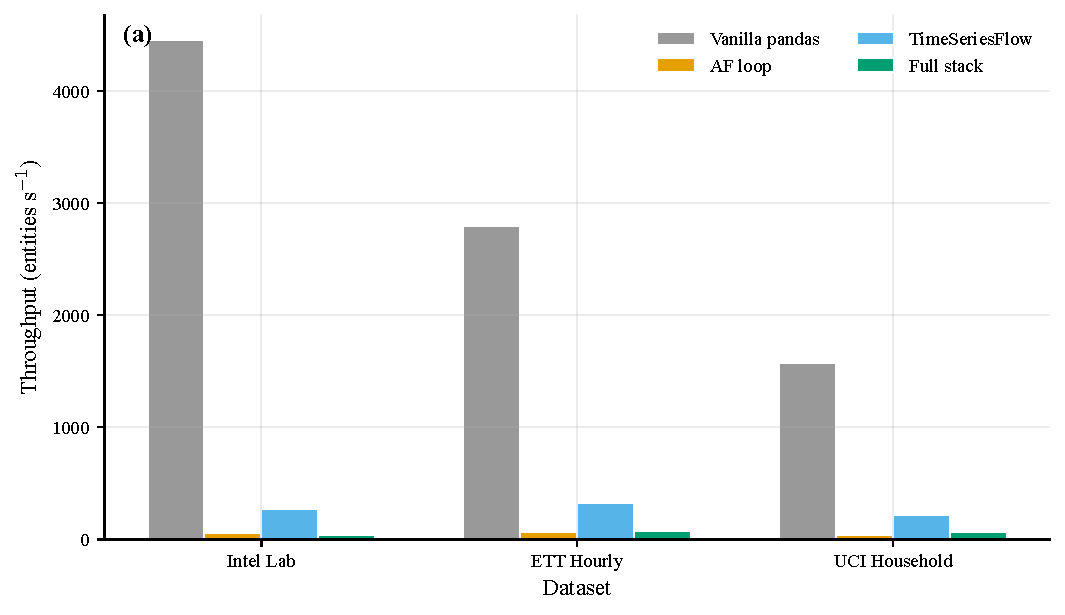
\includegraphics[width=0.95\linewidth]{figures/fig01_throughput.pdf}
  \caption{Entity throughput across datasets and processing approaches. Vanilla pandas maximizes raw speed; the full stack trades throughput for profiling and routing.}
  \label{fig:throughput}
\end{figure}

\begin{figure}[htbp]
  \centering
  \begin{subfigure}[b]{0.48\linewidth}
    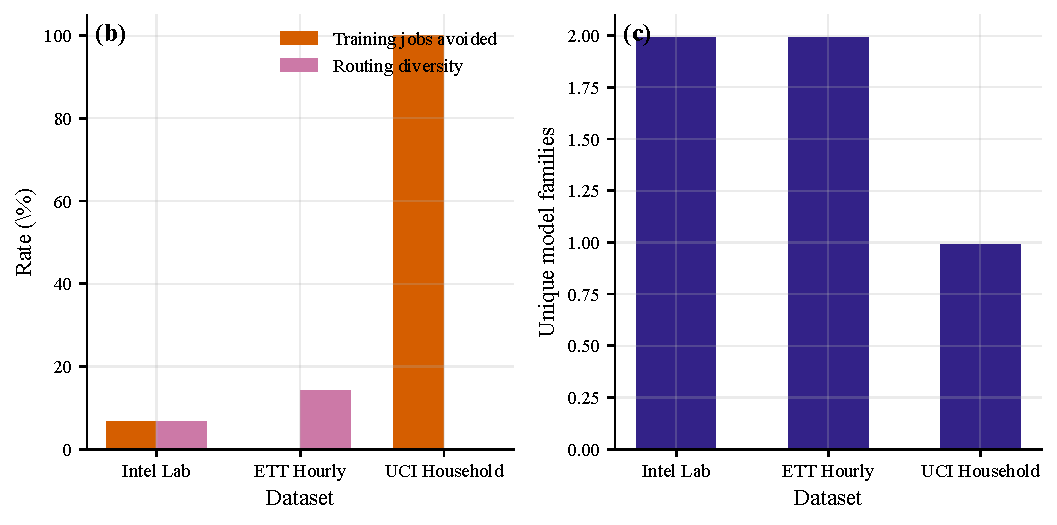
\includegraphics[width=\linewidth]{figures/fig02_commercial_kpis.pdf}
    \caption{Training jobs avoided, routing diversity, and unique model families.}
    \label{fig:commercial}
  \end{subfigure}
  \hfill
  \begin{subfigure}[b]{0.48\linewidth}
    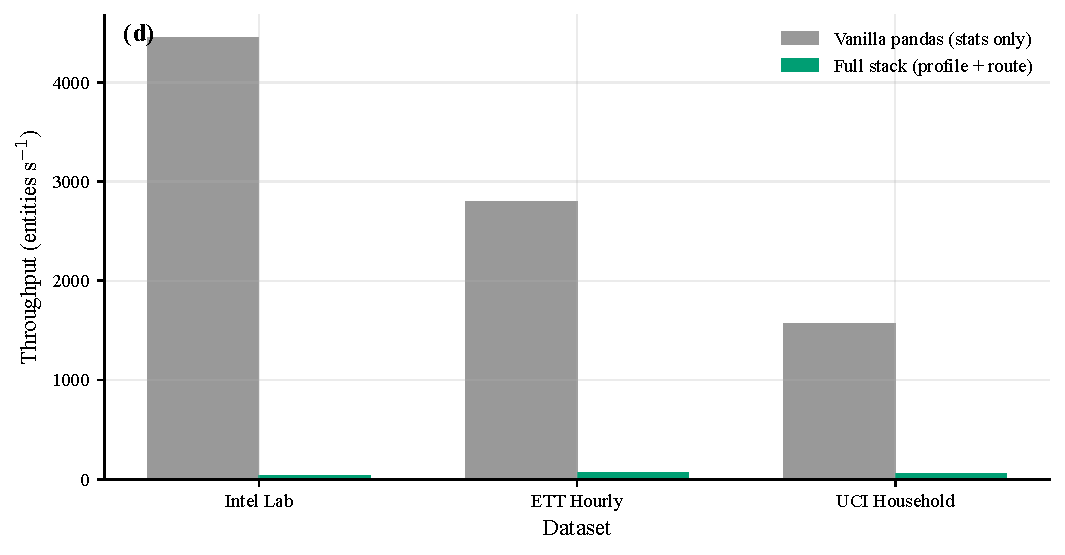
\includegraphics[width=\linewidth]{figures/fig03_screening_throughput.pdf}
    \caption{Vanilla stats throughput versus full-stack screening throughput.}
    \label{fig:screening}
  \end{subfigure}
  \caption{Commercial impact and throughput trade-off.}
\end{figure}

\begin{figure}[htbp]
  \centering
  \begin{subfigure}[b]{0.48\linewidth}
    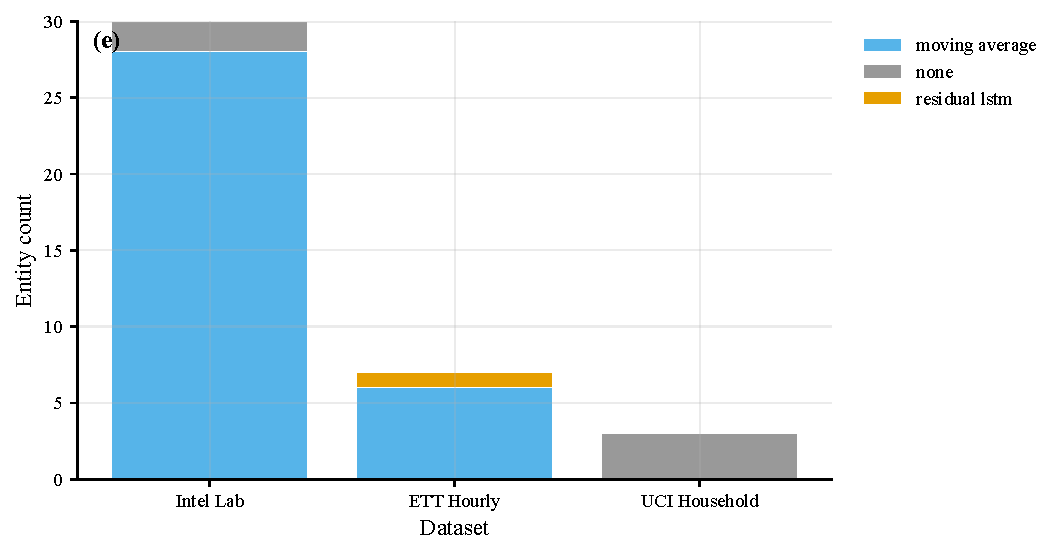
\includegraphics[width=\linewidth]{figures/fig04_model_distribution.pdf}
    \caption{Per-dataset model family assignment counts.}
    \label{fig:models}
  \end{subfigure}
  \hfill
  \begin{subfigure}[b]{0.48\linewidth}
    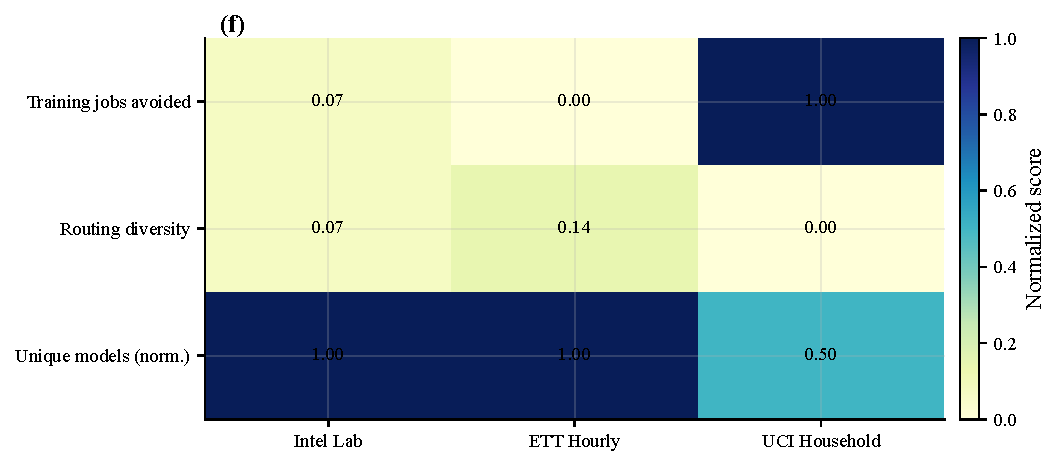
\includegraphics[width=\linewidth]{figures/fig05_kpi_heatmap.pdf}
    \caption{Normalized KPI heatmap across datasets.}
    \label{fig:heatmap}
  \end{subfigure}
  \caption{Routing outcomes and cross-dataset KPI comparison.}
\end{figure}

\section{Per-dataset benchmark tables}

\subsection{Intel Berkeley Lab}
Classic wireless sensor network with 54 motes and irregular sampling intervals.

\begin{tabular}{lrrrr}
\toprule
Approach & Seconds & Entities/s & Gate pass & Routing diversity \\
\midrule
vanilla\_pandas & 0.01 & 4480.31 & --- & --- \\
adaptiveforecast\_loop & 0.56 & 53.80 & 93.3\% & 6.7\% \\
timeseriesflow & 0.16 & 188.98 & --- & --- \\
full\_stack & 0.66 & 45.37 & 93.3\% & 6.7\% \\
\bottomrule
\end{tabular}

\vspace{0.3cm}
\noindent Entities: 30. Rows: 114372. Median rows/entity: 4000. Span (days): 4.8.

\subsection{ETT Hourly (ETTh1)}
Seven electricity transformer load channels on an hourly grid.

\begin{tabular}{lrrrr}
\toprule
Approach & Seconds & Entities/s & Gate pass & Routing diversity \\
\midrule
vanilla\_pandas & 0.00 & 2835.20 & --- & --- \\
adaptiveforecast\_loop & 0.11 & 65.59 & 100.0\% & 14.3\% \\
timeseriesflow & 0.02 & 333.33 & --- & --- \\
full\_stack & 0.10 & 72.85 & 100.0\% & 14.3\% \\
\bottomrule
\end{tabular}

\vspace{0.3cm}
\noindent Entities: 7. Rows: 28000. Median rows/entity: 4000. Span (days): 166.6.

\subsection{UCI Household Power}
Three residential sub-meter channels with minute-level power readings.

\begin{tabular}{lrrrr}
\toprule
Approach & Seconds & Entities/s & Gate pass & Routing diversity \\
\midrule
vanilla\_pandas & 0.00 & 1940.44 & --- & --- \\
adaptiveforecast\_loop & 0.08 & 36.99 & 0.0\% & 0.0\% \\
timeseriesflow & 0.01 & 223.07 & --- & --- \\
full\_stack & 0.05 & 60.64 & 0.0\% & 0.0\% \\
\bottomrule
\end{tabular}

\vspace{0.3cm}
\noindent Entities: 3. Rows: 12000. Median rows/entity: 4000. Span (days): 2.8.


\section{Discussion}
The executive verdict above is the primary takeaway. The sections below provide supporting metrics.

\textbf{How to read throughput charts.}
Do not treat vanilla pandas throughput as a forecast baseline. It computes mean and row count only.
Full-stack throughput reflects profiling plus routing plus orchestration. Compare TimeSeriesFlow to
pandas for orchestration tax; compare full stack to AdaptiveForecast-only for runner overhead.

\textbf{Commercial framing.}
Lead with screening and routing when entity quality varies. Lead with orchestration when batch
reliability matters. Do not sell on pandas speed. Phase 2 must add forecast error metrics before
claiming model-selection effectiveness.

\section{Conclusions}
\begin{itemize}
  \item TimeSeriesFlow: Effective as an orchestration layer (14x slower than pandas on the same lightweight stats task; acceptable overhead for batch structure).
  \item AdaptiveForecast: Partially effective: screening blocks unfit entities before training; routing assigns multiple model families where patterns differ; on UCI Household Power all entities failed gates (short span slice; screening-only outcome). Forecast accuracy was not tested.
  \item Full stack: Partially effective when combines screening with batch orchestration and delivers per-entity routing in one pass at \textasciitilde{}60 entities/s (+0.02s mean vs AdaptiveForecast-only loop). Not faster than pandas; value is operational plus screening, not speed.
  \item Across 40 entities, TimeSeriesFlow is an orchestration layer (\textasciitilde{}14x pandas on stats-only work), AdaptiveForecast adds screening and routing on Intel Berkeley Lab, ETT Hourly (ETTh1), and forecast accuracy remains unmeasured. UCI Household Power blocked every entity under current gates (screening worked; not a deployment-ready forecast slice). Full-stack screening averages 60 entities/s.
\end{itemize}

\vspace{0.5cm}
\noindent Report generated by TimeSeriesFlow open benchmark tooling. Figures exported at 300 DPI with vector PDF companions.

\end{document}
